\chapter{Interviews Documentation \label{cha:interviews}}

This appendix provides the supporting documents used in the study of \LLLs
requirements described in Chapter \ref{cha:model}. The following documents are:

\begin{itemize}
  \item Scenarios used in interviews with lecturers.
  \item Questions used in interviews with lecturers.
  \item Scenarios used in interviews with students.
  \item Questions used in interviews with students.
\end{itemize}

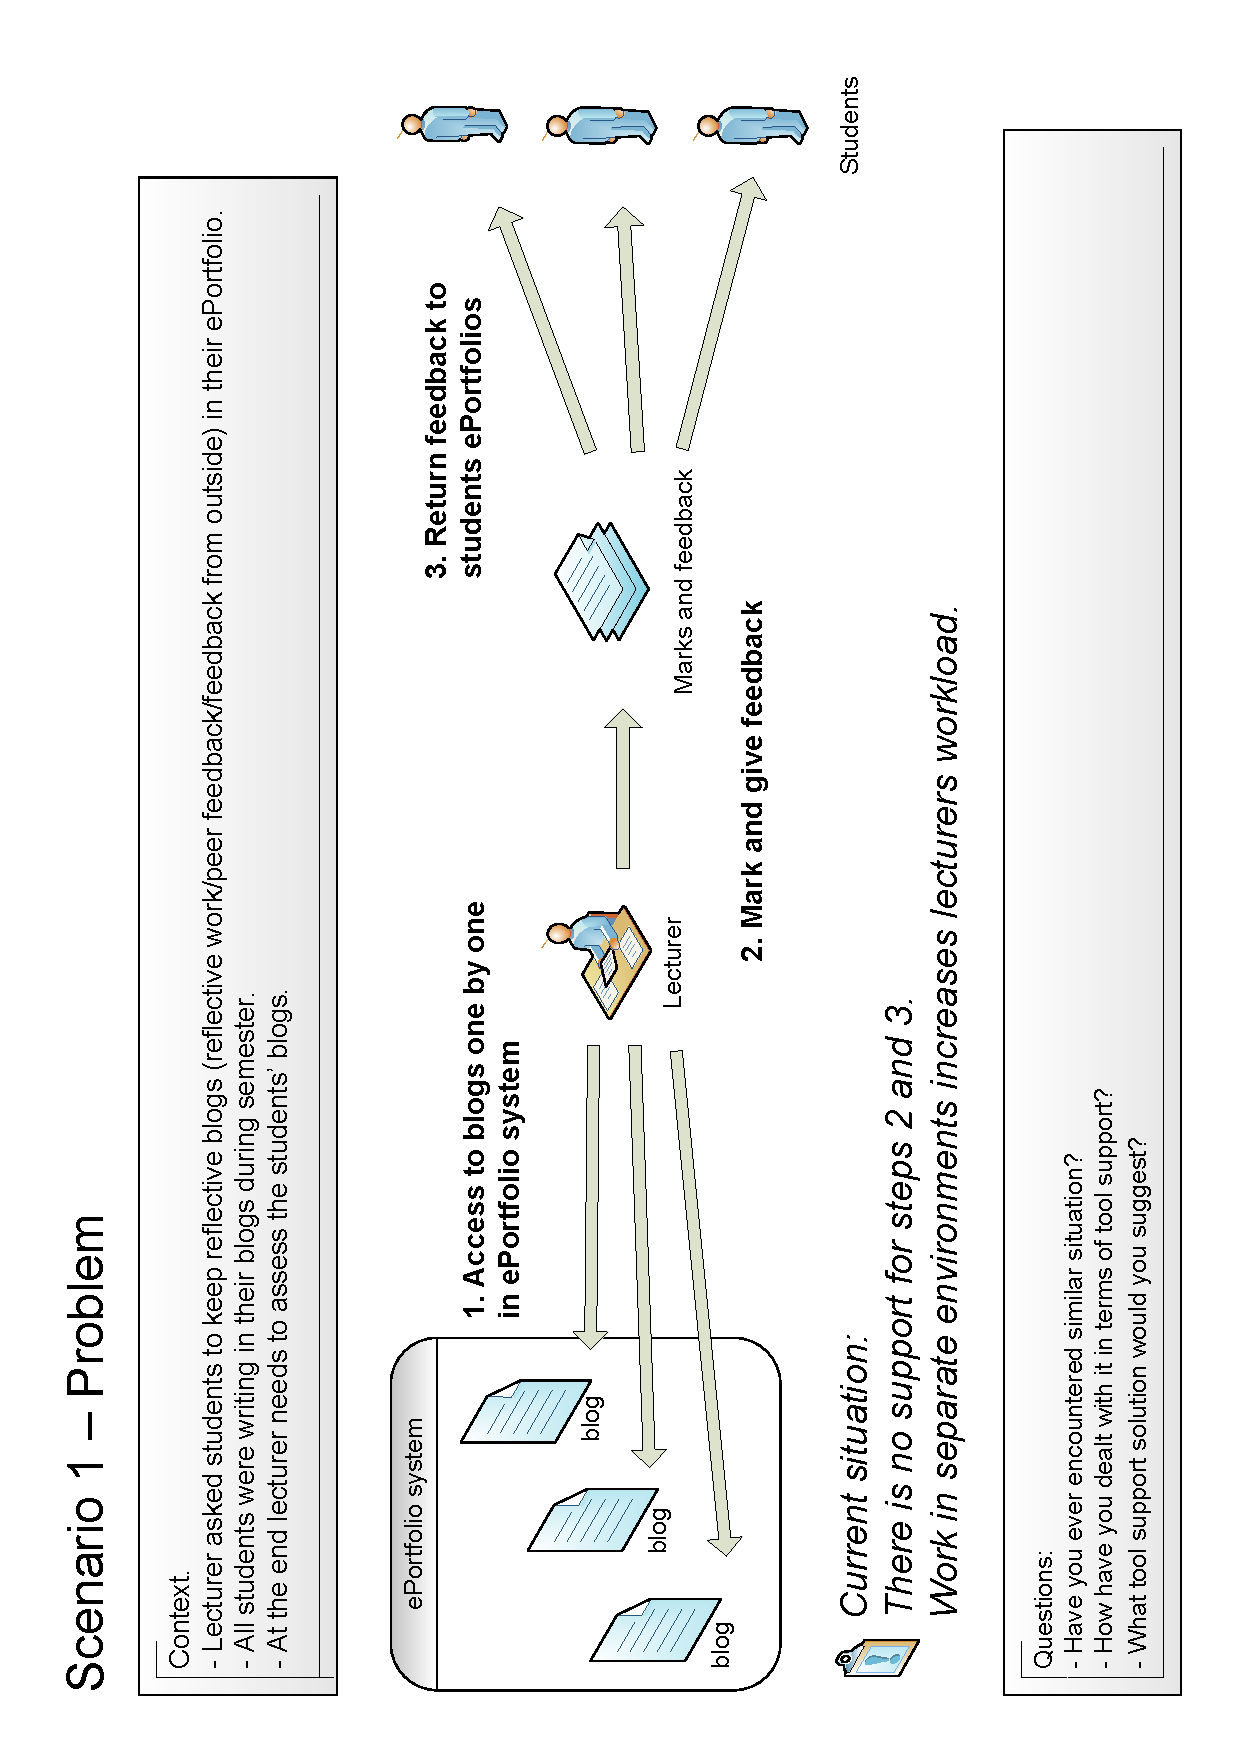
\includepdf[scale=0.7,pages=1,pagecommand=\section{Lecturer Scenario
Examples}\label{sec:appscenariolect},frame]{appendix/Scenarios_L.pdf}

\includepdf[scale=0.75,pages=2,pagecommand={},frame]{appendix/Scenarios_L.pdf}

\includepdf[scale=0.75,pages=3,pagecommand={},frame]{appendix/Scenarios_L.pdf}

\includepdf[scale=0.75,pages=4,pagecommand={},frame]{appendix/Scenarios_L.pdf}

\section{Questions used in the interviews with lecturers}
\label{sec:appquestlect}
\begin{itemize}
\item What is your role as a teacher within the ePortfolio system in the
university?

\item What is your experience of using LMS and ePortfolio systems with students
at university?

\item What do you see as the biggest problems or inefficiencies with using these
systems?

\item Can you describe some specific areas of strengths and weaknesses of
ePortfolio system you have used?

\item What do you think you need to be able to accept an ePortfolio system? What
would be your conditions for its use by students?

\item Looking at LMS from a different perspective, could you add anything to it
which is outside its core functionality that would support students in lifelong
learning?

\item What would you like to do that ePortfolio does not allow you to do now, so
that it could become more useful and relevant to lifelong learning support in
universities?

\item What would you expect a system designed for supporting lifelong learning
provide for students?

\item What other features would you like to see in environments which support
students in lifelong learning in universities?

\item To sum up, we discussed such features as \ldots. Which of them do you
think are the most important for a student-centred lifelong learning environment?
\end{itemize}

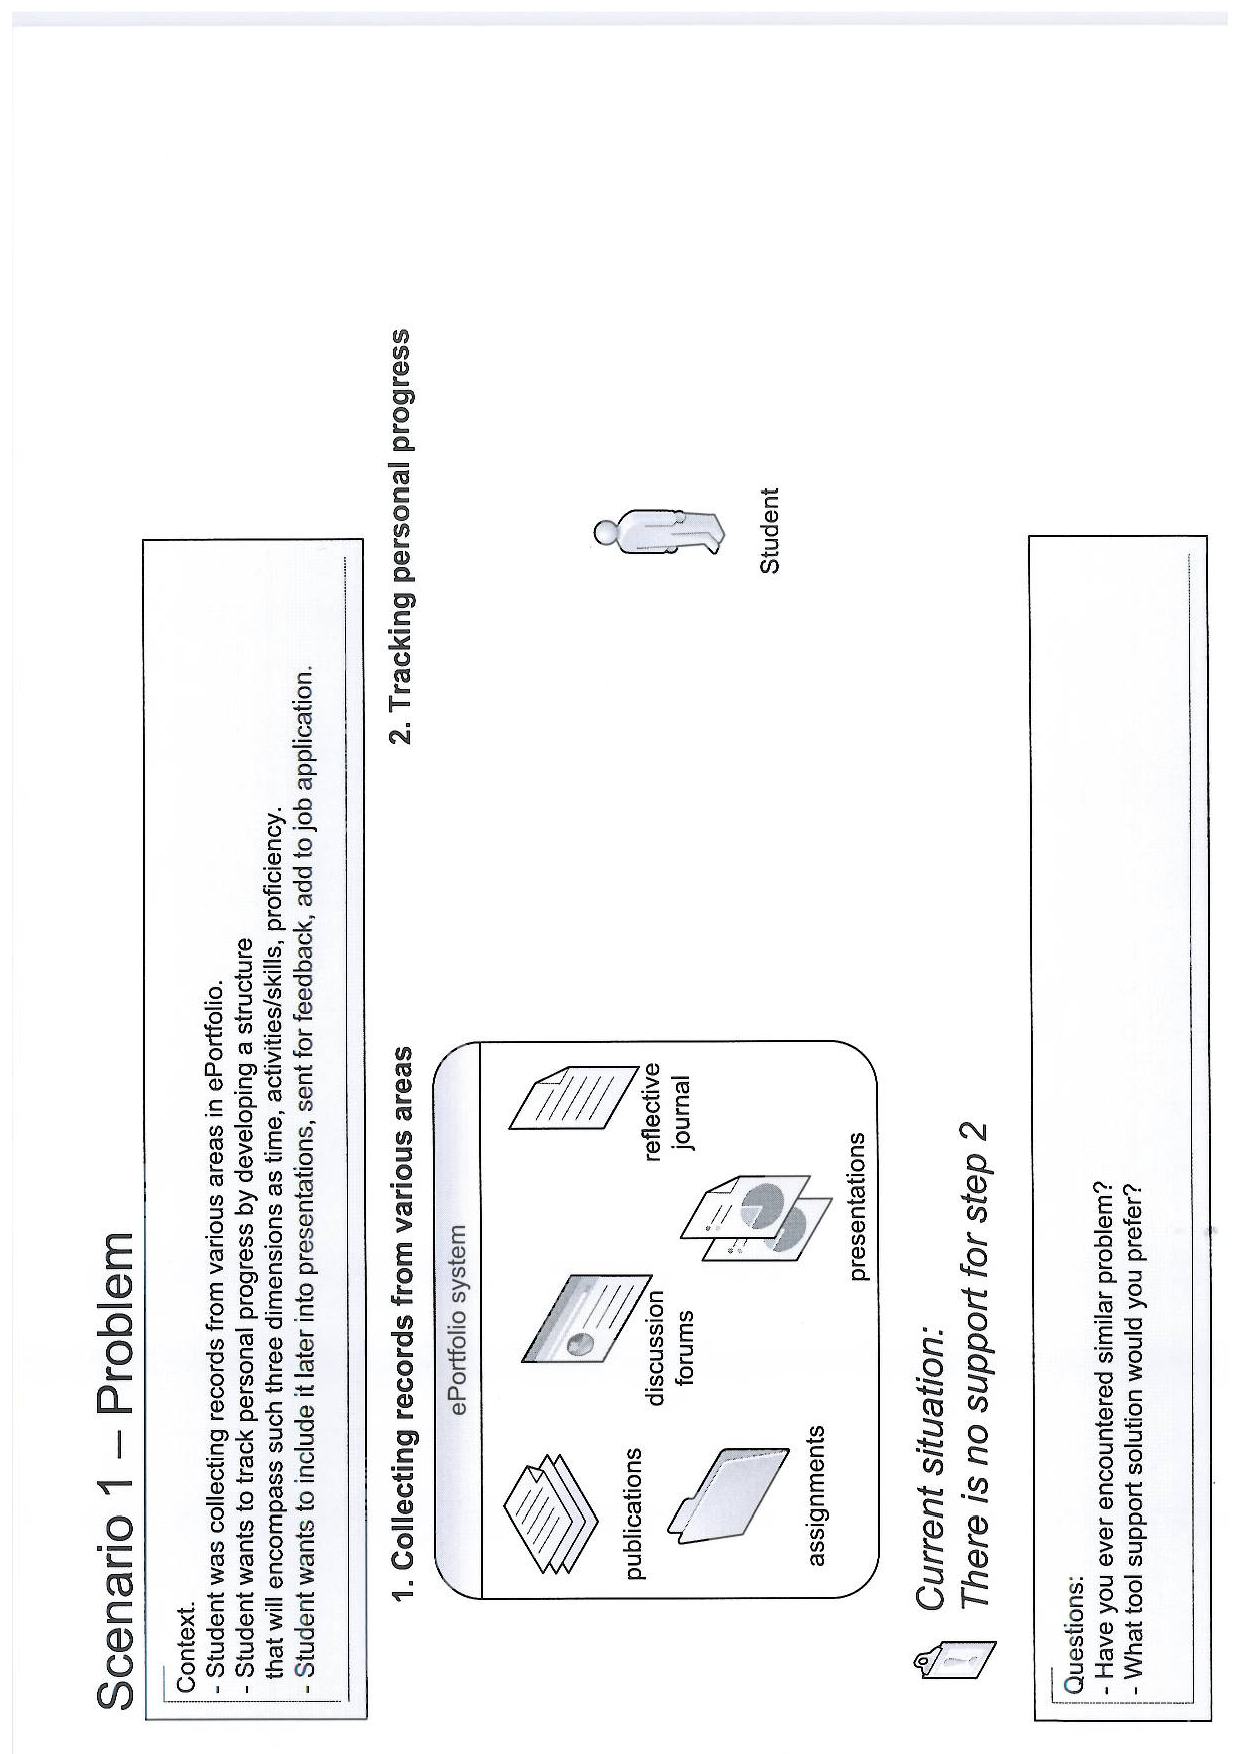
\includepdf[scale=0.7,pages=1,pagecommand=\section{Student Scenario
Examples}\label{sec:appscenariostud},frame]{appendix/Scenarios_S.pdf}

\includepdf[scale=0.75,pages=2,pagecommand={},frame]{appendix/Scenarios_S.pdf}

\includepdf[scale=0.75,pages=3,pagecommand={},frame]{appendix/Scenarios_S.pdf}

\includepdf[scale=0.75,pages=4,pagecommand={},frame]{appendix/Scenarios_S.pdf}

\includepdf[scale=0.75,pages=5,pagecommand={},frame]{appendix/Scenarios_S.pdf}

\section{Questions used in the interviews with students}
\label{sec:appqueststud}
\begin{itemize}
\item 

\item 

\item 

\item 

\item 

\end{itemize}